\subsection{Part 1: Building PCB}
\begin{enumerate}

\item Go to GitHub Repository and save all the .gbr files under the Air-Quality-PCB folder. 

\begin{figure}[h]
    \centering
    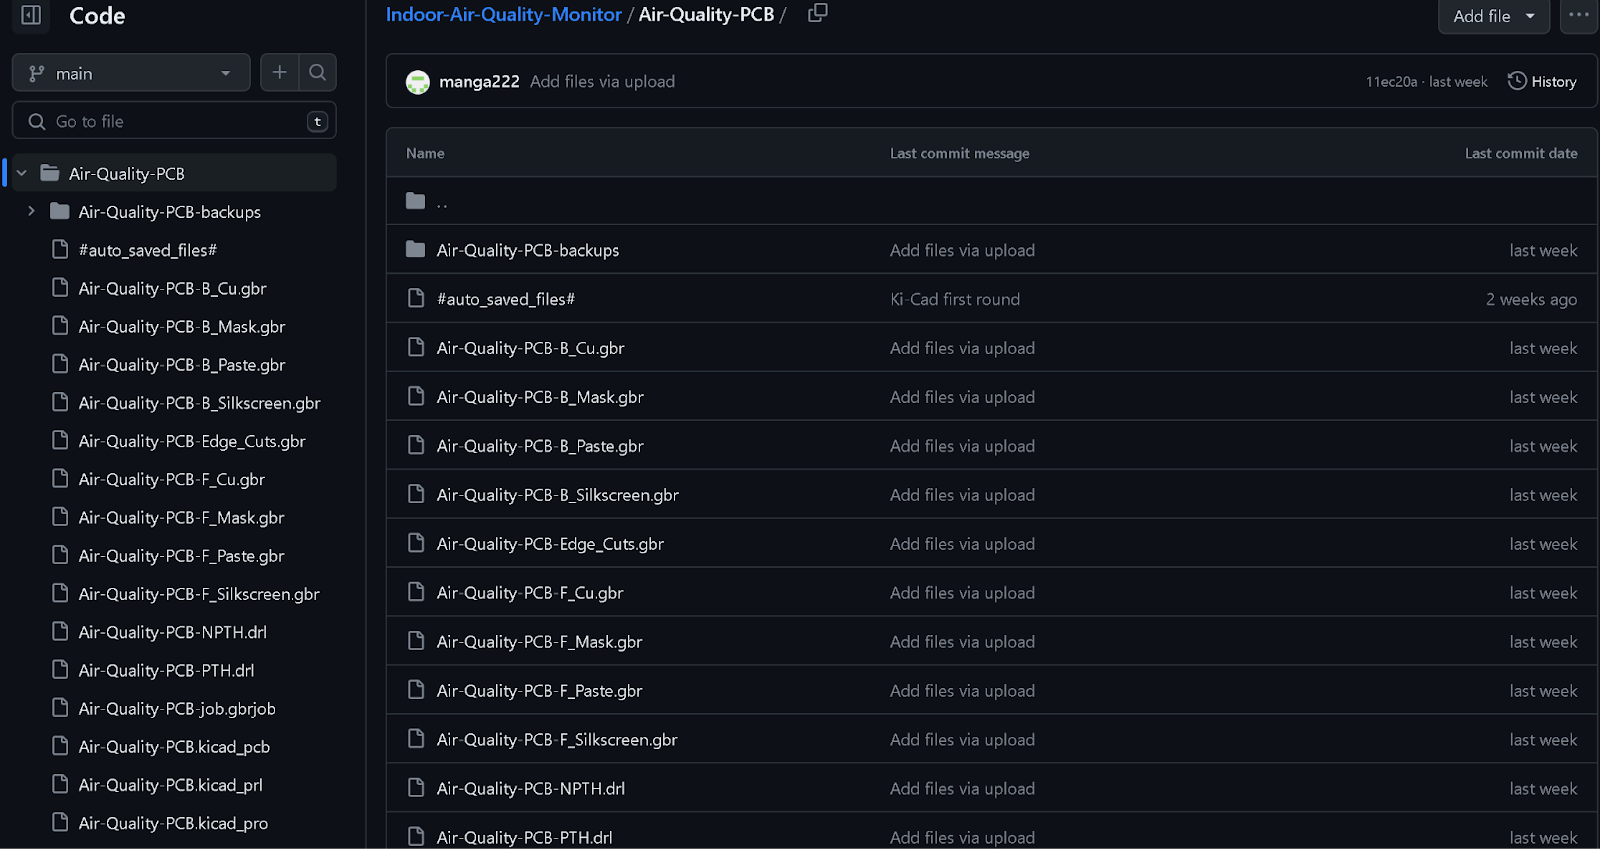
\includegraphics[width=0.8\textwidth]{Pictures/image (7).png}
    \caption[GitHub Repository]{GitHub Repository} 
    \label{fig:part1commrin}
\end{figure}

\item Open the website of your PCB manufacturer and go to their ordering page
\item We used JLCPCB for the project as they were the cheapest and fastest at the time. Link can be found in the project resources section
\item Drag and drop all the .gbr files 
\item Select your options 
\item We selected the default options at time but chose to go with faster delivery 
\item Solder on connection points so the MSP430 can be seated onto the PCB
\item Solder pins onto powerboost charger as well as the 3.3V converter 
\item We ended up removing LED (power and Low indicators) since they consumed too much power and were always on
\end{enumerate}

\subsection{Part 2: Building Enclosure}
\begin{enumerate}

\item Using a laser cutter, cut out the file \texttt{box\_v2.dxf}. It is designed to be cut out of $\frac{1}{{8}}$ inch thick acrylic, but any other $\frac{1}{{8}}$ inch thick material should work. For different thickness materials, the enclosure would have to be redesigned. For reference, a 16 inch x 24 inch sheet is enough to cut out parts for one enclosure. Alternatively, a pre-built plastic enclosure of a similar size could be used, with holes cut for sensors at the same size as our enclosure holes.
\item The batteries and anemometer must be placed as far away from the PM2.5 and CO$_2$ sensor as possible. 
\item The PM2.5 and CO$_2$ must be mounted at the bottom of the enclosure to ensure that they are not susceptible to particle build up. Mount the PM2.5 sensor so that the green side is facing out and away from the wall when mounted.
\item Hot glue the sides of the enclosure while placing the components in the box as it is being assembled. Do not hot glue the lid on. Use clear tape to secure the lid.
\end{enumerate}

\subsection{Part 3: Mounting the Enclosure}
\begin{enumerate}
    \item Once the enclosure build is complete, attach 4 Command Picture Hanging Velco Strips, 1 to each corner of the back wall of the enclosure.
    \item Select a wall to mount enclosure to. For the Anemometer enclosure, mount the unit near air source or vent. For enclosures without an anemometer, mount away from doors, windows or vents. Mount enclosures without anemometers approximately 4-6 feet above ground. 
    \item When batteries need to be changed, detach system. Reattach system when batteries are replaced by again securing system to wall via velcro. 
\end{enumerate}